\documentclass[12pt, a4paper]{article}

\usepackage[a4paper, margin=2cm]{geometry}
\usepackage{setspace}
\usepackage[portuguese]{babel}
\usepackage{graphicx}
\usepackage{hyperref}
\usepackage{amsfonts}

\chardef\_=`_

\title{\textbf{LI3 - Relatório da Fase I - Grupo 12}}
\author{
    Humberto Gomes (A104348) \\
    José Lopes     (A104541) \\
    José Matos     (A100612) \\
}
\date{novembro de 2023}

\begin{document}
\maketitle
\onehalfspacing
\setlength{\parskip}{\baselineskip}
\setlength{\parindent}{0pt}

\begin{abstract}
    Este relatório tem como intuito explicar a estrutura do nosso trabalho prático para a UC de LI3.
    O foco principal desta UC é a modularização e o encapsulamento do código, logo, este documento
    descreve como tal foi conseguido, justificando as nossas decisões a este nível. Esta 1.ª fase do
    projeto foca-se no \emph{parsing} e validação de um \emph{dataset} contendo utilizadores, voos,
    passageiros destes e, por fim, reservas de hotéis, sobre o qual serão executadas \emph{queries}.
    Nesta fase, apenas estão implementadas seis, fornecendo informação sobre a base de dados. O
    modo de organização e processamento destes dados também está descrito neste documento.
\end{abstract}

\section{Estrutura do trabalho}

Devido à elevada complexidade e ao elevado número de módulos neste projeto, segue um diagrama de
dependências completo, que será depois separado em diversas secções lógicas, que têm o seu
funcionamento descrito uma a uma. Contudo, para reduzir a complexidade visual, não incluímos
todas as relações de dependência, mas apenas as mais relevantes. É, então, apresentada a
nossa convenção gráfica:

\begin{itemize}
    \item Um retângulo com cantos arredondados representa uma estrutura de dados;
    \item Um retângulo sem cantos arredondados representa um módulo cuja tarefa principal é a
          execução de código. Porém, alguns destes módulos pode conter estruturas de dados
          auxiliares (por exemplo, uma gramática definida no módulo de um \emph{parser});
    \item $A \rightarrow B$ significa que o módulo $A$ depende do módulo $B$. $A \dashrightarrow B$
          representa uma falsa dependência, por exemplo, a necessidade de se saber da existência
          de um nome de um tipo opaco.
\end{itemize}

\begin{figure}[ht]
    \centering
    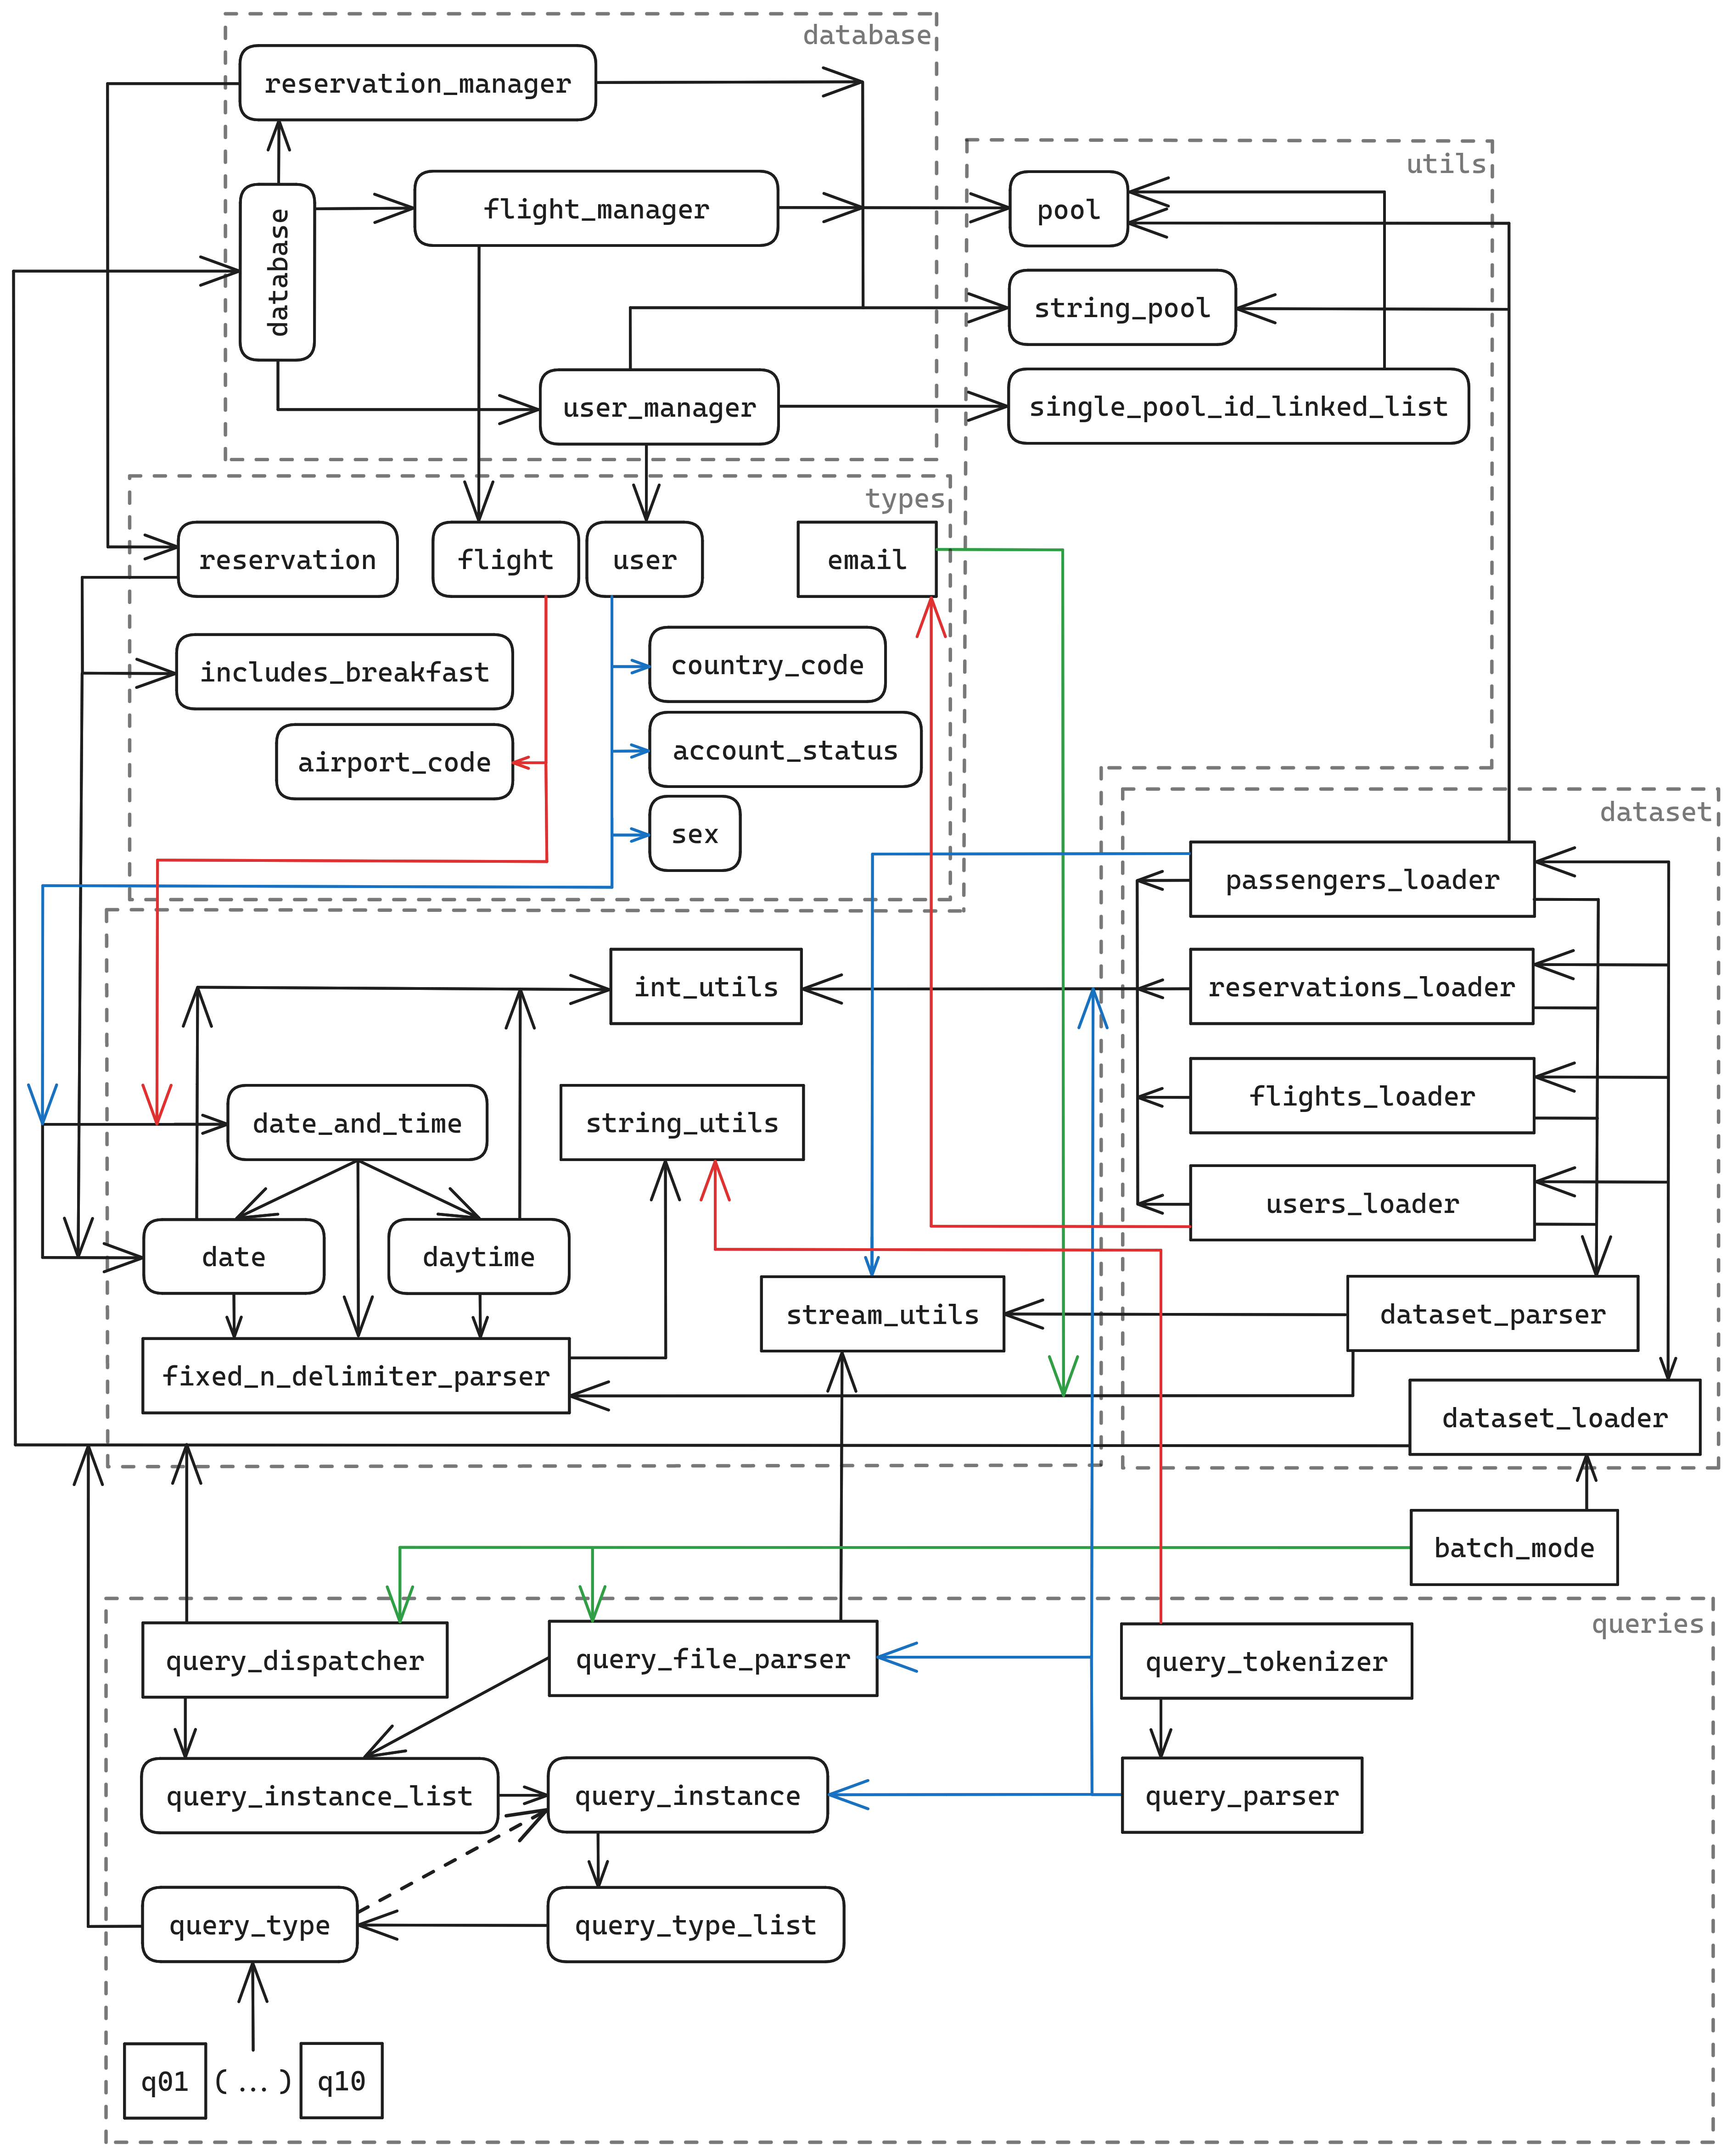
\includegraphics[scale=0.10]{res-fase1/full_dependency_graph.png}
    \caption{Diagrama de dependências de toda a aplicação. Cores são utilizadas apenas para
             facilitar a leitura.}
    \label{fig:diagram}
\end{figure}

\subsection{\emph{Parsing}}
\label{sec:parsing}

\begin{figure}[ht]
    \centering
    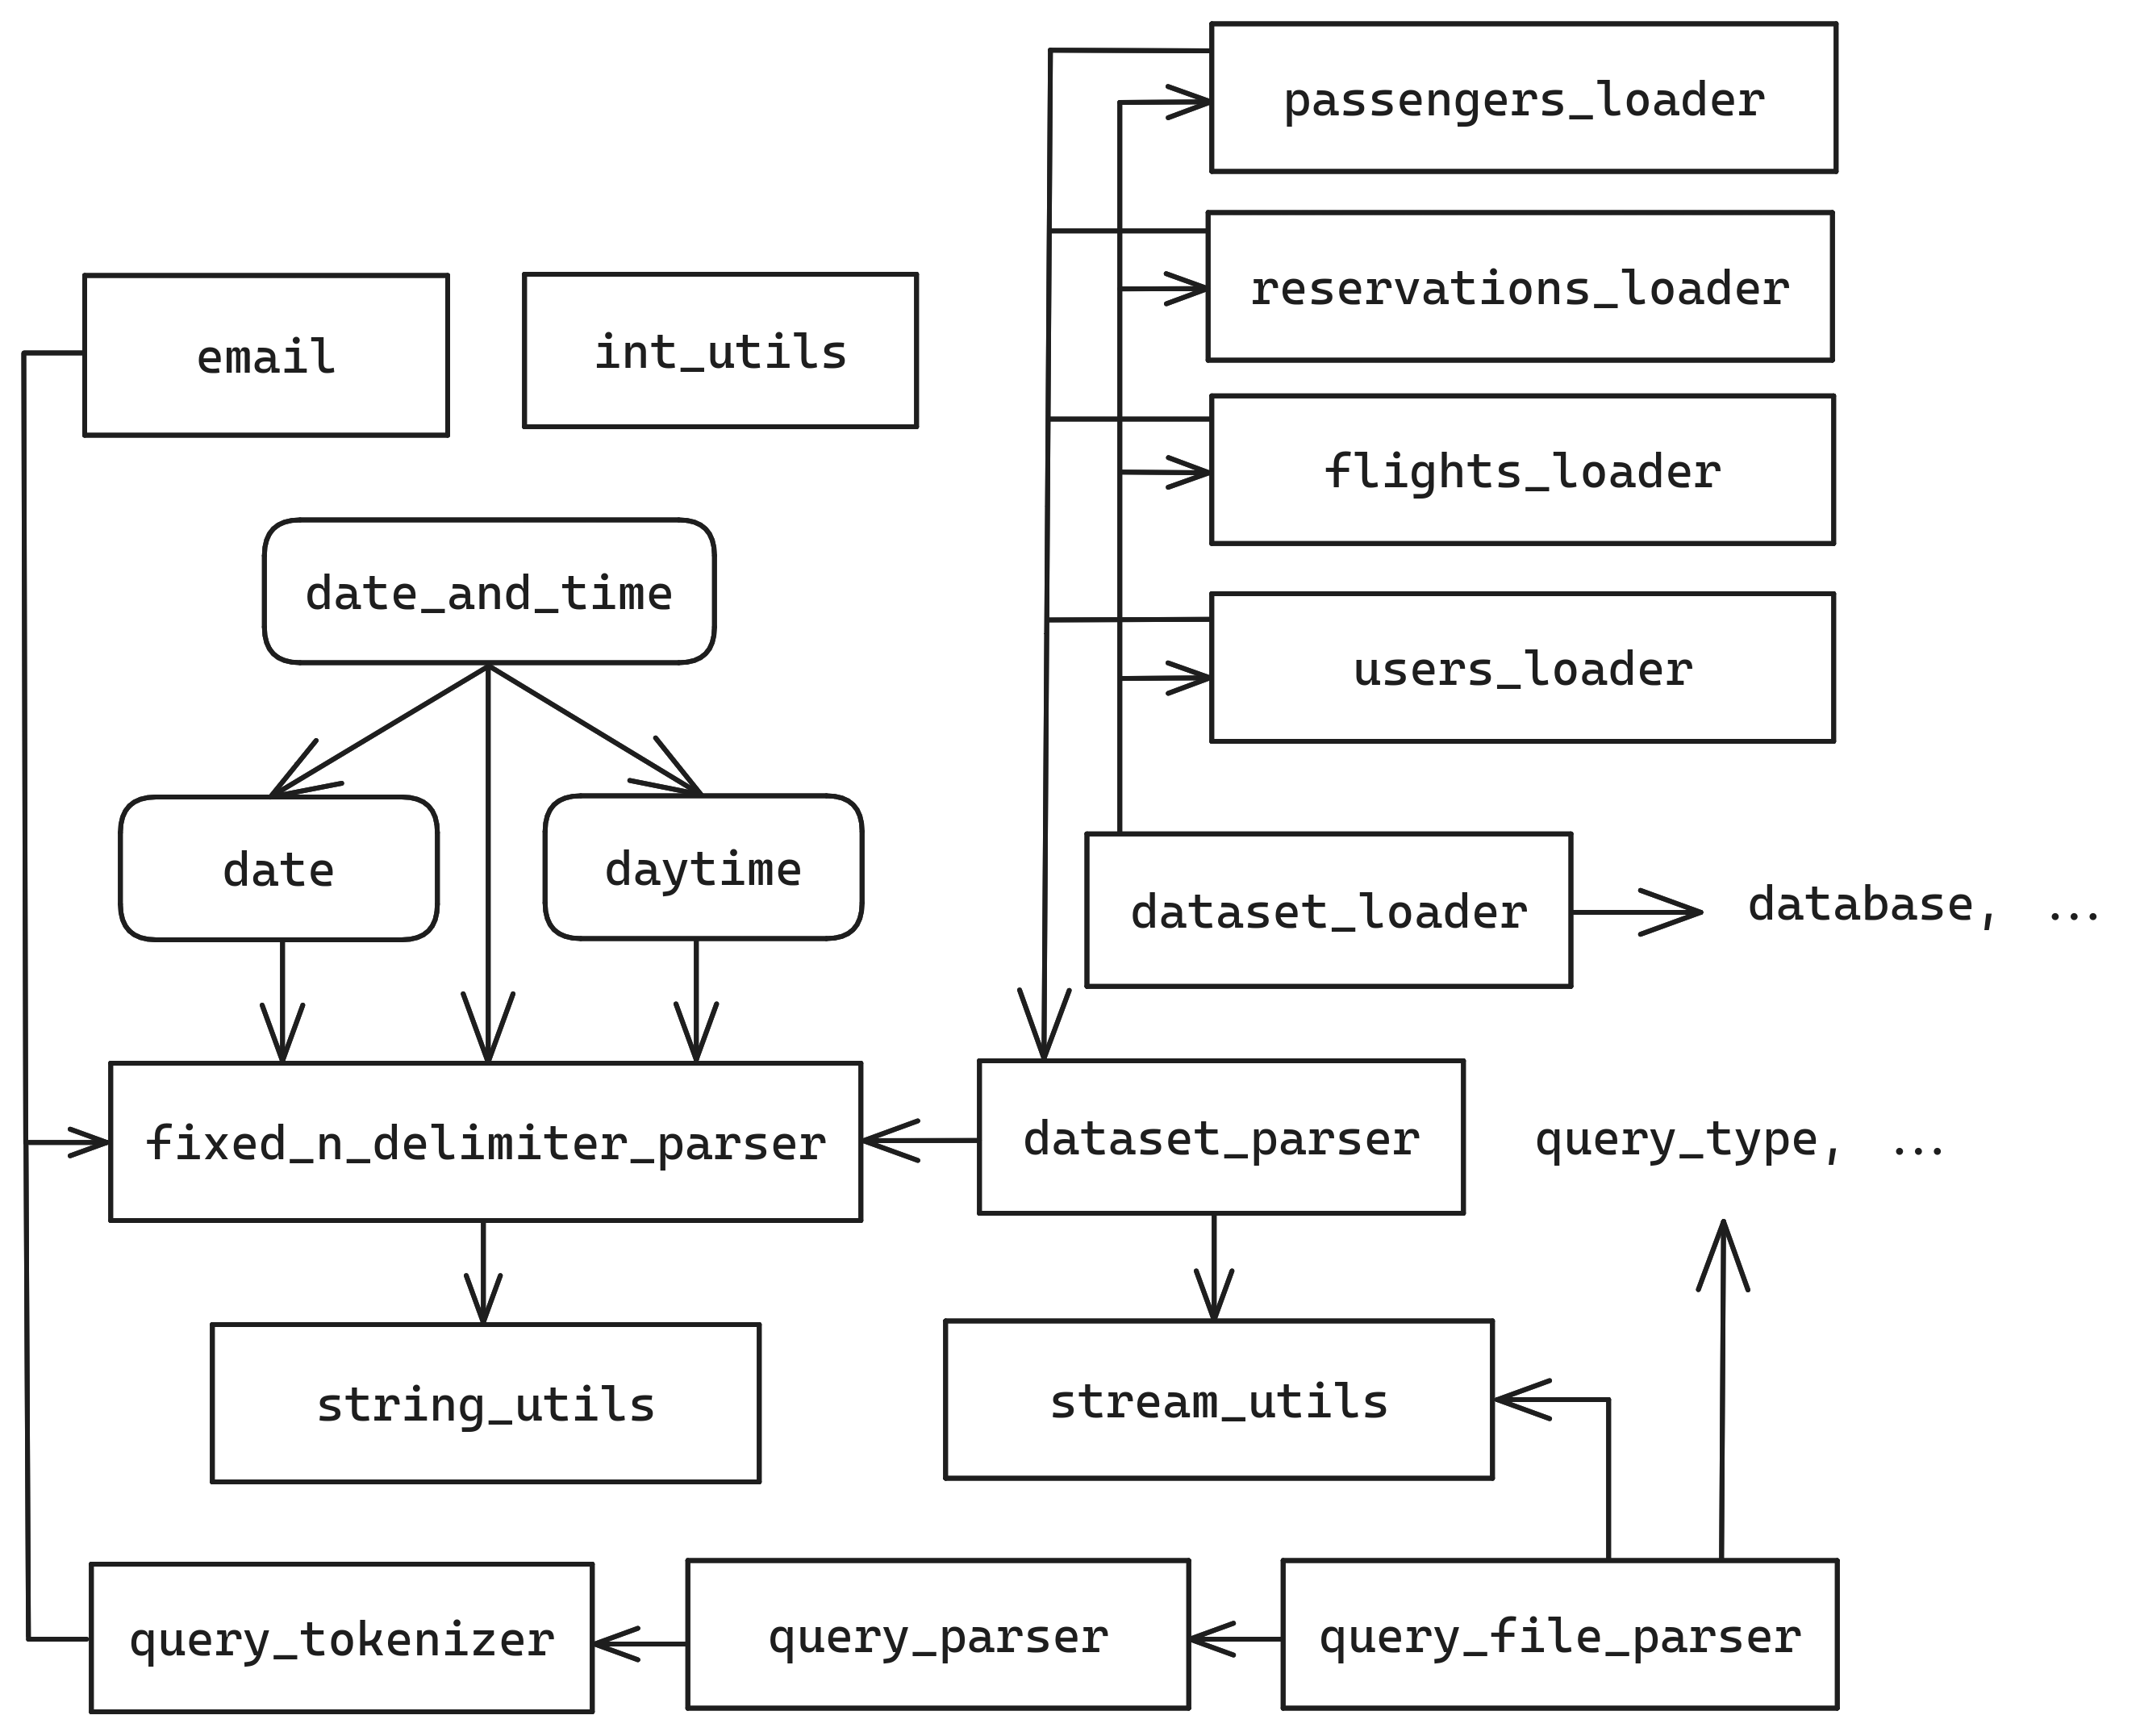
\includegraphics[scale=0.17]{res-fase1/parsing.png}
    \caption{Diagrama de dependências do subsistema de \emph{parsing}}
    \label{fig:parsing}
\end{figure}

O nosso sistema de \emph{parsing} começa com \emph{tokenizadores}, que separam \emph{strings} e
ficheiros por um delimitador (\texttt{string\_utils} e \texttt{stream\_utils}, respetivamente).
Sobre estes é construído o caso mais específico do \texttt{fixed\_n\_delimiter\_parser}, que espera
um número pré-determinado de \emph{tokens}, chamando um \emph{callback} diferente para cada um; uma
gramática genérica, definida pelo programador, que contém estes \emph{callbacks}. Este \emph{parser}
é utilizado tanto para a validação de \emph{emails} (\texttt{email}), como para o \emph{parsing} de
datas (\texttt{date}), horas de um dia (\texttt{daytime}), combinações de datas e horas
(\texttt{date\_and\_time}), e linhas de um \emph{dataset}. Por fim, \texttt{int\_utils} é um
\emph{parser} de valores inteiros, semelhante às funções \texttt{atoi} e \texttt{strtol}, mas com
uma melhor deteção de erros.

Para a análise dos ficheiros de um \emph{dataset}, o \texttt{dataset\_parser} é responsável por
separar o ficheiro por linhas, excluir a primeira linha (o \emph{header} da tabela CSV) e
\emph{tokenizar} cada linha, chamando os \emph{callbacks} adequados na sua gramática, também
customizável. O \texttt{dataset\_loader}, não propriamente encaixado neste secção de
\emph{parsing}, é responsável por abrir cada ficheiro do \emph{dataset} e interagir com os
\emph{parsers} adequados (\texttt{*\_loader}), que adicionam elementos à base de dados. Ao mesmo
tempo, o \texttt{dataset\_loader} regista os erros reportados nos ficheiros de erro.

O \emph{parsing} de \emph{queries} requer um \emph{tokenizador} adicional para lidar com aspas
(\texttt{query\_tokenizer}), um \emph{parser} para determinar o tipo de uma \emph{query} e se os
seus argumentos são válidos (\texttt{query\_parser}), e um \emph{parser} de um ficheiro com uma
\emph{query} por linha (\texttt{query\_file\_parser}).

\subsection{Entidades}
\label{sec:entities}

\begin{figure}[ht]
    \centering
    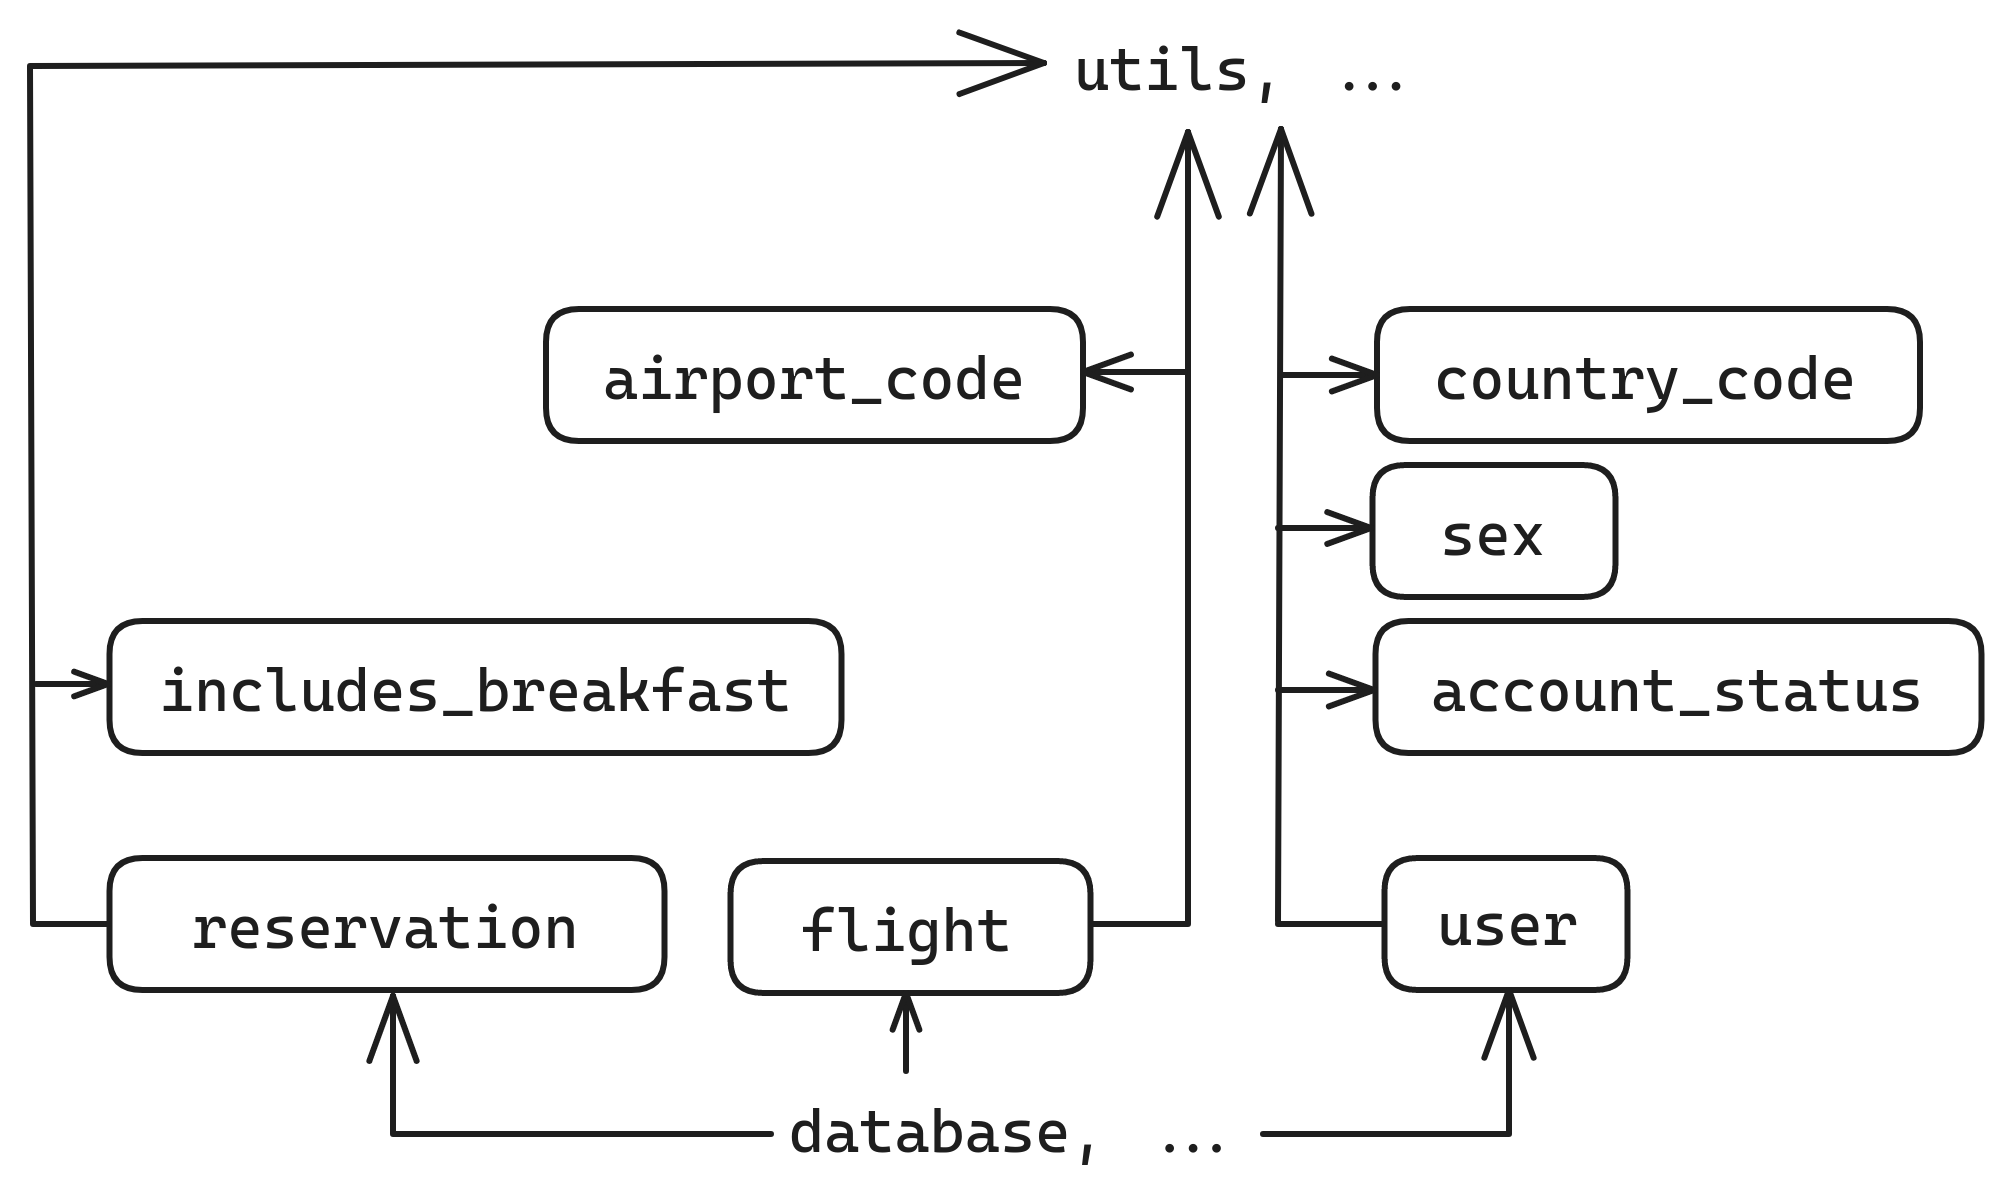
\includegraphics[scale=0.2]{res-fase1/entities.png}
    \caption{Diagrama de dependências das entidades da aplicação}
    \label{fig:entities}
\end{figure}

O nosso projeto define três entidades (\texttt{user\_t}, \texttt{reservation\_t} e
\texttt{flight\_t}), correspondentes às definidas no enunciado do trabalho, juntamente com módulos
de estruturas de dados auxiliares. Os campos destas entidades formam um subconjunto dos campos
definidos no enunciado do trabalho (não armazenamos campos nunca pedidos por \emph{queries}). A
única exceção ocorre nos voos, onde adicionamos um campo relativo ao número de passageiros, devido
à sua grande utilidade tanto para a validação do \emph{dataset} como para a execução de
\emph{queries}.

\subsection{Catálogos}
\label{sec:catalogs}

Antes de definirmos uma base de dados, começámos por definir estruturas que permitem melhorar a
eficiência espacial e a velocidade das alocações na aplicação: um alocador em \texttt{pool} para
objetos todos do mesmo tamanho, e uma \texttt{string\_pool} para \emph{strings}. Definimos também
uma \texttt{single\_pool\_id\_linked\_list}, uma implementação de uma lista ligada na qual que
várias listas podem partilhar a mesma \texttt{pool} para armazenamento de nodos, contribuindo para
um menor uso de memória em \emph{overheads} de alocação.

\begin{figure}[ht]
    \centering
    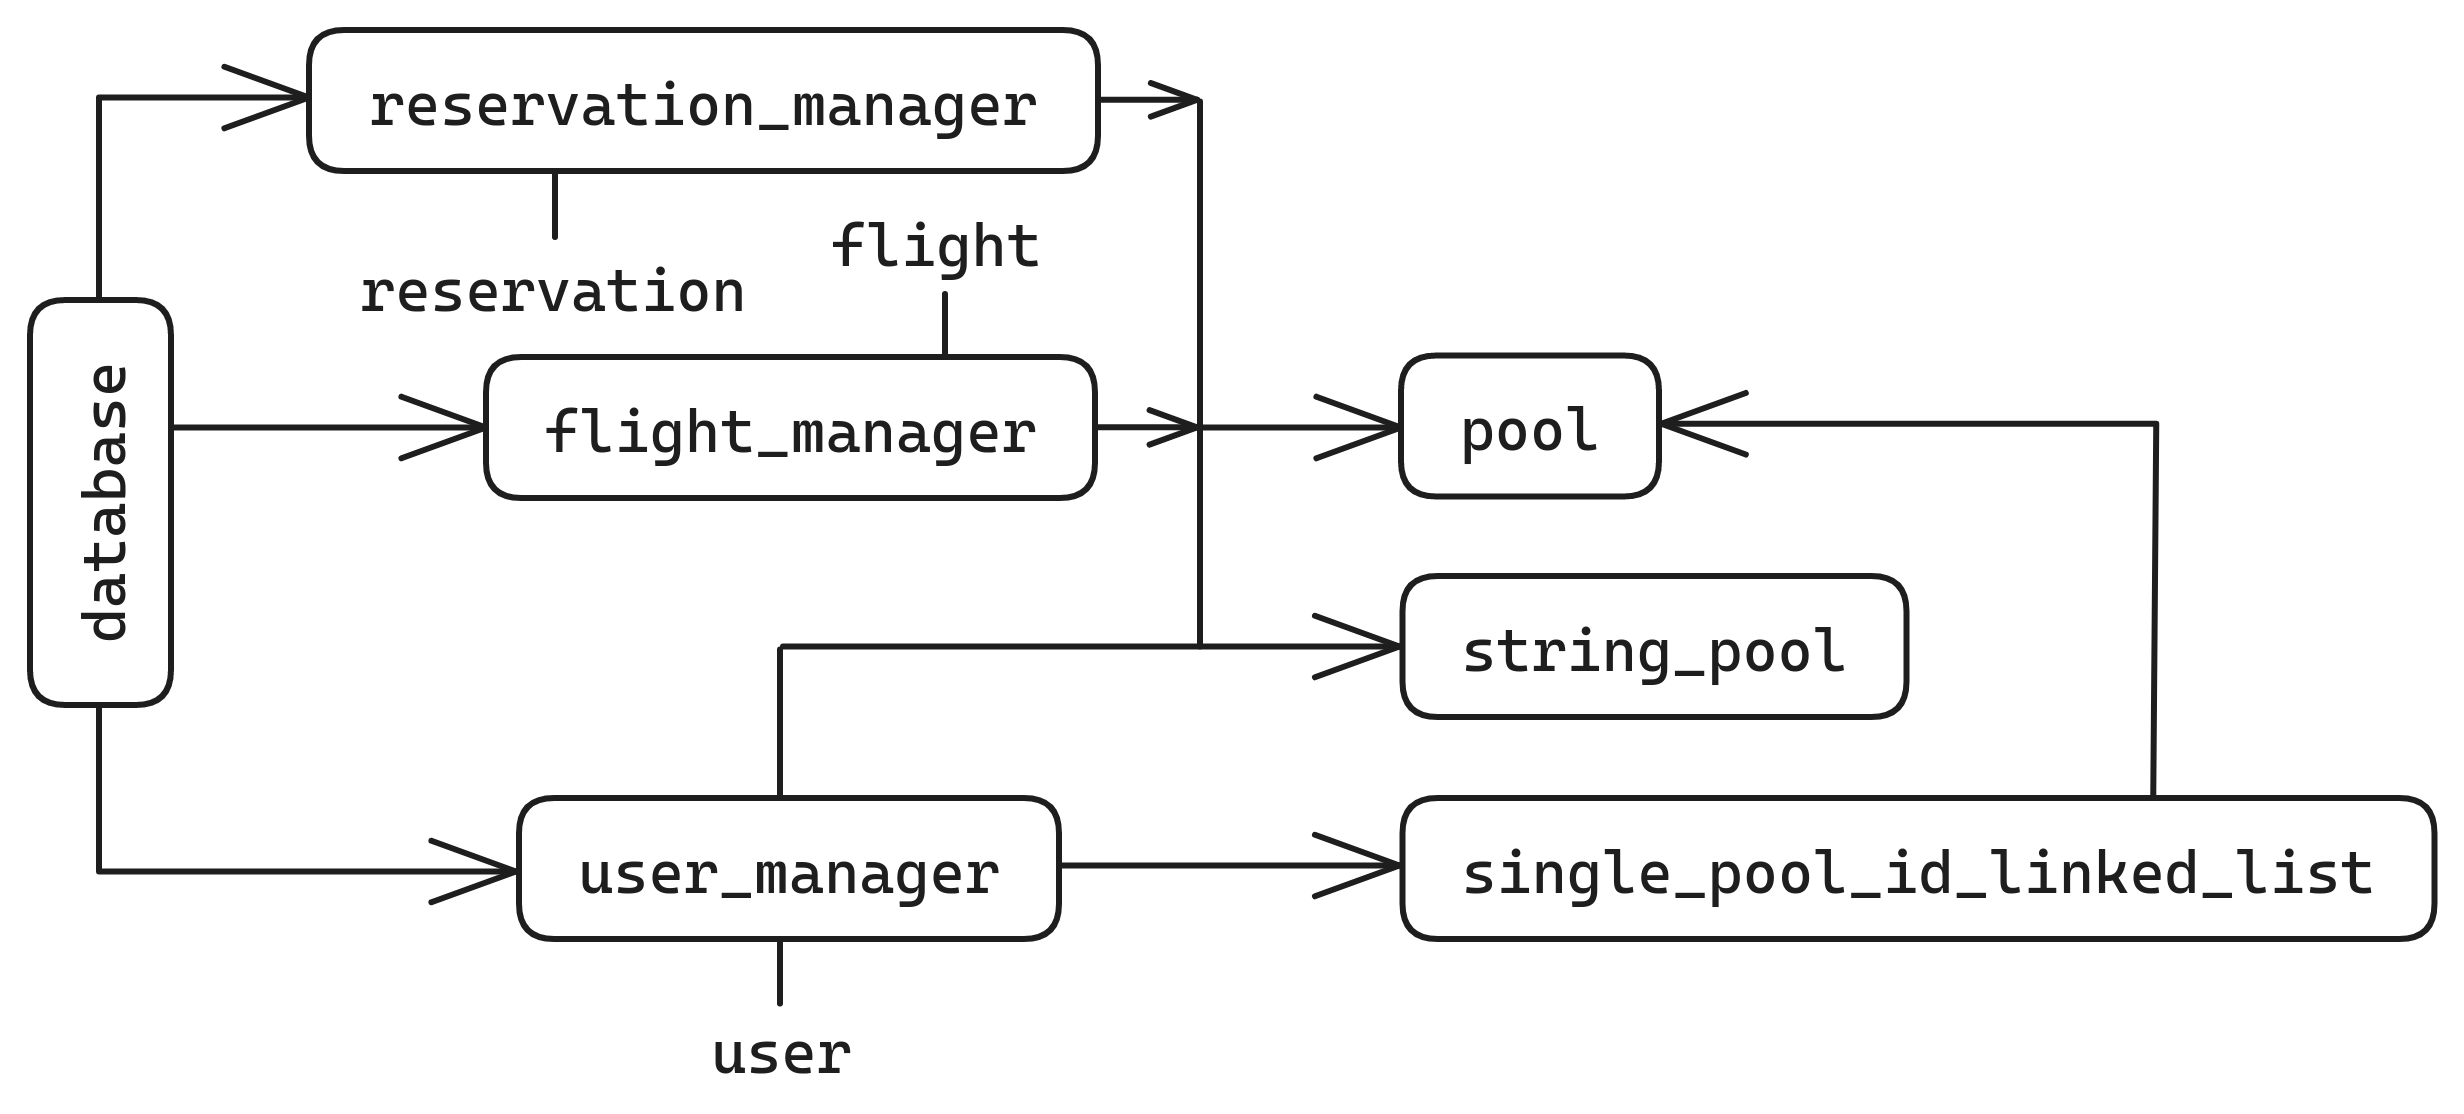
\includegraphics[scale=0.2]{res-fase1/database.png}
    \caption{Diagrama de dependências dos catálogos na aplicação}
    \label{fig:catalogs}
\end{figure}

No módulo \texttt{database}, definimos uma estrutura de dados que contém os três \emph{managers} na
aplicação: o \texttt{reservation\_manager}, que gere as reservas; o \texttt{flight\_manager}, que
gere voos; e o \texttt{user\_manager}, que gere utilizadores. Este último liga também cada
utilizador aos identificadores de voos e reservas a ele associados. Todos estes \emph{managers}
consistem numa \texttt{pool} para alocação de entidades, uma \texttt{string\_pool} para alocação de
\emph{strings}, e uma tabela de \emph{hash}, para a associação de identificadores de entidades às
entidades em si. O \texttt{user\_manager} surge como exceção, onde cada identificador de um
\texttt{user} se encontra também associado a listas ligadas com os IDs dos voos e reservas
associados a esse utilizador.

\subsection{\emph{Queries}}
\label{sec:queries}

O \emph{parsing} de \emph{queries} já foi descrito na secção \nameref{sec:parsing}. No sistema de
\emph{queries}, começámos por definir um \texttt{query\_type}, um conjunto de \emph{callbacks} que
define um tipo de \emph{query}, de modo a simular polimorfismo em C. Definir uma \emph{query}
resume-se a definir uma função para cada \emph{callback}, e adicioná-la à
\texttt{query\_type\_list}, a lista de todas as \emph{queries} conhecidas.

Antes de enumerar as \emph{queries} implementadas, devemos mencionar como geramos dados estatísticos
para uma \emph{query}. Ao contrário do sugerido no enunciado no projeto, não utilizamos um módulo
para estatísticas, dado que implementá-lo seria uma quebra do modularidade da aplicação: implementar
uma nova \emph{query} implicaria edições consideráveis a vários módulos. Sendo assim, optámos por um
modelo em que dados estatísticos são gerados por cada tipo (número) de \emph{query}, e são
partilhados por todas as \emph{queries} do mesmo tipo. Por exemplo, torna-se possível fazer uma
única iteração da base de dados para todas as \emph{queries} do tipo 3, em vez de uma iteração para
cada \emph{query} deste tipo. Assim, temos uma solução mais modular, mas com pior desempenho do que
um módulo de estatísticas globais (que faria uma única iteração pelos dados, gerando dados usados
por todas as \emph{queries}).

\begin{figure}[ht]
    \centering
    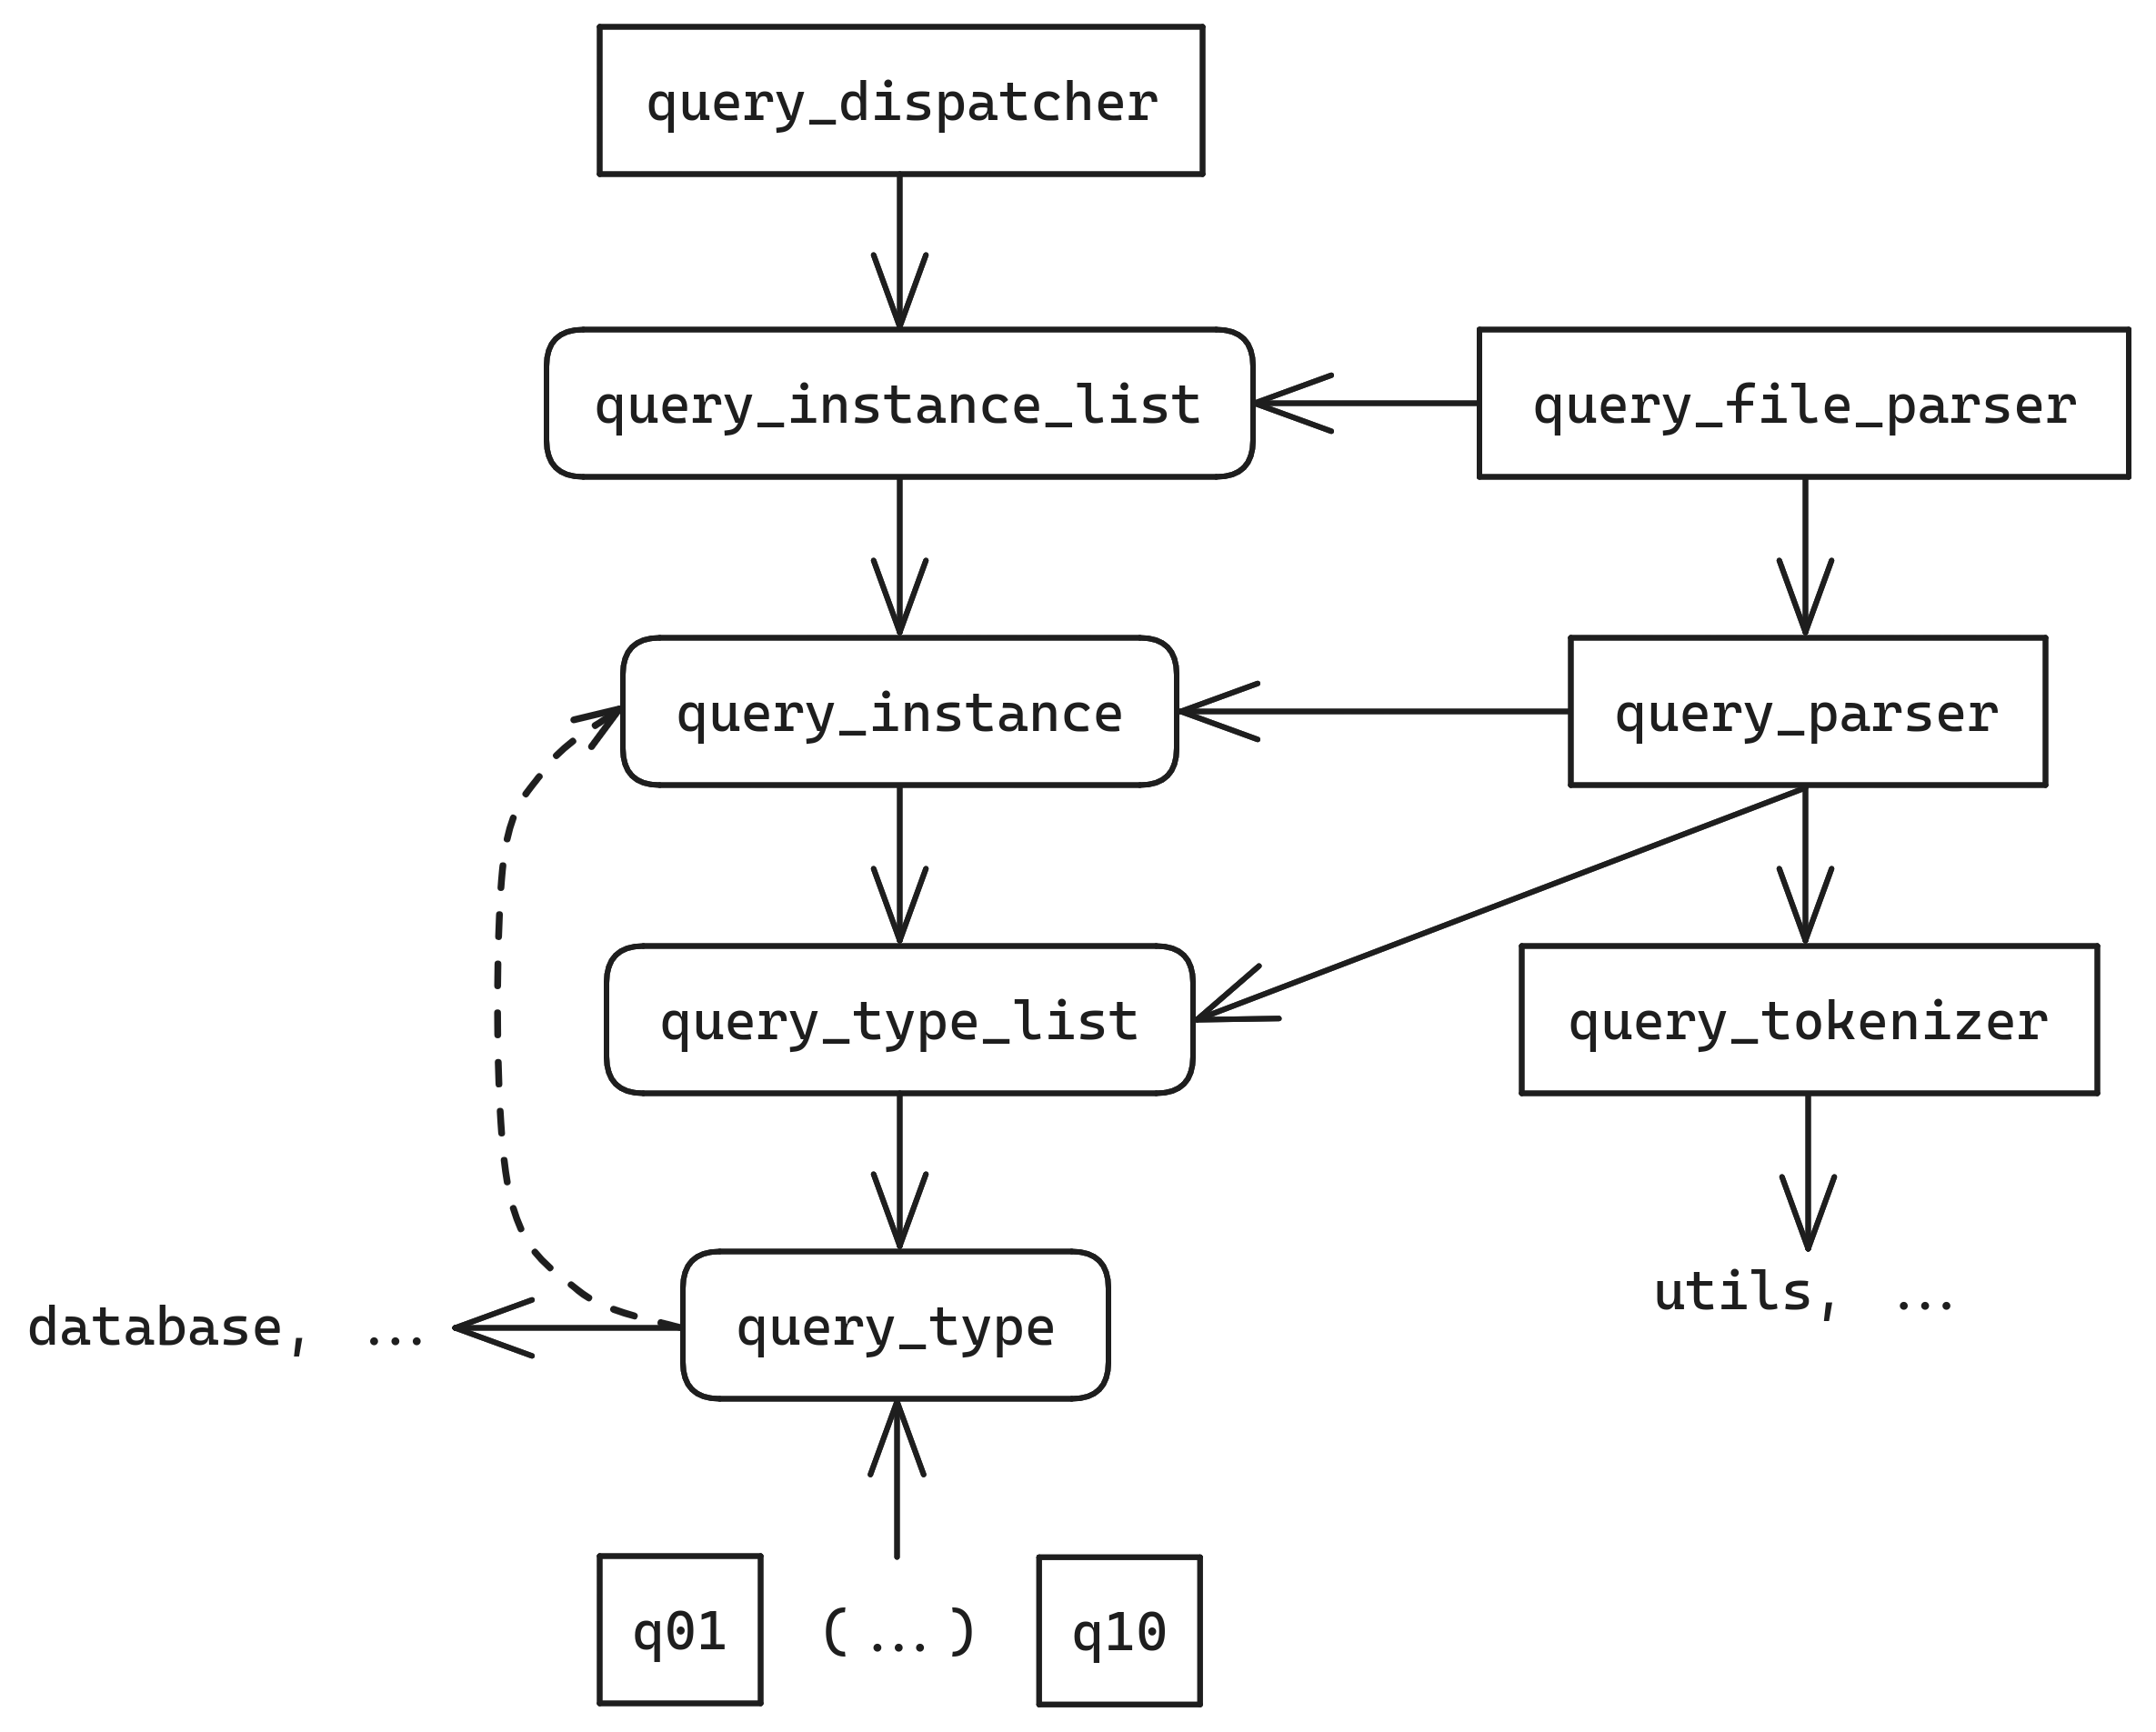
\includegraphics[scale=0.19]{res-fase1/queries.png}
    \caption{Diagrama de dependências do subsistema de \emph{queries}}
    \label{fig:queries}
\end{figure}

Estas são as \emph{queries} que implementámos nesta primeira fase:

\begin{itemize}
    \item \textbf{Q01} - Consulta de uma entidade pelo seu identificador. A sua implementação foi
                         trivial: começa-se por determinar o tipo da entidade com base no formato
                         do seu identificador, processo seguido da consulta direta do \emph{manager}
                         correto na base de dados.

    \item \textbf{Q02} - Listagem de voos e / ou reservas de um utilizador. Também de implementação
                         trivial, esta \emph{query} pede a lista de reservas / voos (ou ambas) de um
                         utilizador ao \texttt{user\_manager} (consulta direta), seguida da consulta
                         também direta do \emph{manager} adequado para cada voo / reserva, para a
                         obtenção de informação sobre data do evento.

    \item \textbf{Q03} - Apresentação da classificação média de um hotel. Numa única iteração
                         estatística pelas reservas, calcula-se a média de todos os hotéis
                         mencionados nas \emph{queries} de tipo 3. A execução de cada \emph{query}
                         resume-se então à consulta direta dos dados estatísticos, formados por uma
                         tabela de \emph{hash} que associa o identificador de um hotel à sua média.

    \item \textbf{Q04} - Listagem das reservas de um hotel. Tal como a Q03, faz-se uma única
                         iteração estatística da lista de reservas, mas em vez de se calcular uma
                         média com cada reserva, adiciona-se a reserva a um \emph{array} associado
                         a esse hotel através de uma tabela de \emph{hash}. Após se ordenar cada
                         \emph{array}, pode-se proceder à execução de cada \emph{query}, que
                         consiste numa consulta direta dos dados estatísticos.

    \item \textbf{Q06} - Listagem dos $N$ aeroportos com mais passageiros num dado ano. Com uma
                         única iteração estatística pelo \texttt{flight\_manager}, forma-se uma
                         tabela de \emph{hash}, que associa anos a outras tabelas de \emph{hash},
                         que por sua vez associam aeroportos a números de passageiros. Cada uma
                         destas segundas tabelas de \emph{hash} é convertida para um \emph{array}
                         ordenado de pares aeroporto-passageiros. Assim, a execução de uma
                         \emph{query} limita-se à escolha do \emph{array} de pares correto e à
                         apresentação dos seus primeiros $N$ elementos.

    \item \textbf{Q09} - Listagem de todos os utilizadores cujo nome tenha como prefixo o argumento
                         desta \emph{query}. De momento, devido ao breve prazo de entrega,
                         implementámos esta \emph{query} ineficientemente, com uma iteração do
                         gestor de utilizadores e filtragem dos nomes por cada \emph{query} no
                         ficheiro de \emph{input}. Segue-se a ordernação e apresentação dos
                         resultados. Pretendemos melhorar esta \emph{query} na segunda fase,
                         adicionando uma árvore binária de procura com os nomes dos utilizadores
                         ao \texttt{user\_manager}.
\end{itemize}

Retornando à descrição de cada módulo, uma \texttt{query\_instance} refere-se à ocorrência de uma
\emph{query} (num ficheiro, por exemplo), e uma \texttt{query\_instance\_list} a uma lista destas.
Por último, o \texttt{query\_dispatcher} é o módulo responsável por executar uma lista de
\emph{queries} dada uma base de dados e os ficheiros de \emph{output} de cada \emph{query}.

\section{Otimização do uso de memória}

Dado que os \emph{datasets} da 2.ª fase serão de maior dimensão, preocupámo-nos desde já com a
quantidade de memória utilizada, de modo não sermos futuramente obrigados a reescrever partes
significativas do nosso código.

\subsection{Observação do \emph{dataset} e das \emph{queries}}

Podemos observar que alguns campos do \emph{dataset} nunca precisavam de estar presentes no
\emph{output} de nenhuma \emph{query} (ex: o \emph{email} de um utilizador), pelo que era escusado
o seu armazenamento na base de dados, sendo apenas necessária a sua validação durante o
\emph{parsing}. Ademais, por observação dos \emph{datasets} em si, podemos concluir que é possível
armazenar certos campos usando tipos de dados de menor tamanho (ex: o identificador de um voo
pode ser armazenado como um inteiro, em vez de uma \emph{string}).

\subsection{Tipos opacos}

Um dos nossos obstáculos principais foi a forma como tipos opacos são implementados em C, que,
devido à sua natureza de apontador, exigem uma alocação por instância, gerando significativa
ineficiência em \emph{overhead} de alocação. Esta secção descreve como, mantendo o encapsulamento
dos tipos, conseguimos definir tipos de dados opacos sem estas limitações.

\subsubsection{Estruturas de dados com menos de 8 bytes}

Certas estruturas de dados, como datas, horas, códigos de aeroporto, \emph{etc.} contêm menos de
8 bytes de informação. Assim, uma destas estruturas pode ser definida como um inteiro (com o número
de bits adequado), evitando-se uma alocação por cada instância desta estrutura. Os métodos relativos
a essa estrutura de dados usam uma \texttt{union} para aceder aos seus campos, como é visto no
seguinte exemplo para datas:

\begin{spacing}{1}
\begin{center}
    \begin{tabular}{ |l|l| }
        \hline
        \emph{include/utils/date.h}: & \emph{src/utils/date.c}: \\
        & \\
        \texttt{typedef int32\_t date\_t;} & \texttt{typedef union \{} \\
                                           & \texttt{\ \ \ \ date\_t date;} \\
                                           & \texttt{} \\
                                           & \texttt{\ \ \ \ struct \{} \\
                                           & \texttt{\ \ \ \ \ \ \ \ uint16\_t year;} \\
                                           & \texttt{\ \ \ \ \ \ \ \ uint8\_t month, day;} \\
                                           & \texttt{\ \ \ \ \} fields;} \\
                                           & \texttt{\} date\_union\_helper\_t;} \\
        \hline
    \end{tabular}
\end{center}
\end{spacing}

\subsubsection{Alocação de entidades em \emph{pools}}

Como já descrito na secção \nameref{sec:catalogs}, o nosso projeto utiliza alocação em \emph{pools}
de modo a reduzir o \emph{overhead} da alocação genérica de memória. Para tal ser possível com
tipos opacos, cada entidade precisa de ter um método que devolve o seu tamanho, por exemplo,
\texttt{user\_sizeof}.

\section{Destaques e aspetos a melhorar}

O nosso grupo encontra-se satisfeito com o nível de modularidade e abstração que atingimos nesta
primeira fase. Dada a estrutura modular do projeto, é importante que a interface de cada módulo
apresente um comportamento bem documentado. Por isso, todas as estruturas de dados e métodos
encontram-se fartamente documentados, incluindo até exemplos de utilização! Utilizando
\href{https://www.doxygen.nl}{\emph{Doxygen}}, podemos formar páginas HTML com a documentação
formatada, como visível na figura abaixo:

\begin{figure}[ht]
    \centering
    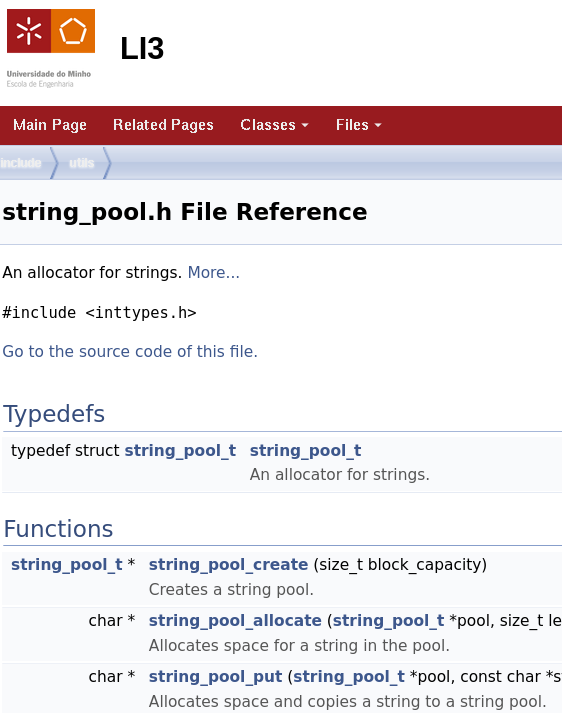
\includegraphics[scale=0.35]{res-fase1/doxygen.png}
    \caption{Índice da documentação do ficheiro \texttt{string\_pool.h} na documentação
             \emph{Doxygen}}
    \label{fig:doxygen}
\end{figure}

Por outro lado, temos noção de que é possível ainda melhorar a modularidade, com a construção de
abstrações sobre algumas estruturas de dados da \emph{glib}. No área do encapsulamento, apesar de
termos definido \emph{getters} e \emph{setters}, fomos recentemente informados pelos docentes que
deveríamos estar a criar cópias dos valores devolvidos, sendo o uso de \texttt{const}, a nossa
solução atual, desaconselhado. Pretendemos implementar essa recomendação para a segunda fase de
entrega.

Ademais, apesar de, à data de escrita deste relatório sermos, na plataforma de teste, entre os
grupos com o trabalho completo, o que usa menos memória, ainda temos algumas ideias de como melhorar
o seu uso para a próxima fase. Por último, as nossas ferramentas de desenvolvimento estão bastante
completas, com um \emph{Makefile} com geração automática de dependências (para diminuir tempos de
compilação), e \emph{scripts} para verificação de \emph{memory leaks} (com supressões), formatação
automática de código, e \emph{profiling}.

\section{Conclusão}

Em suma, nesta primeira fase, procurámos criar alicerces sólidos para a estrutura da nossa
aplicação, sobre os quais poderemos facilmente desenvolver a segunda fase, tirando proveito da
extensibilidade que o desenvolvimento modular tem para oferecer. Estamos confiantes de que o
\emph{dataset} de maior dimensão da 2.ª fase será capaz de caber em memória com as nossas estruturas
de dados, mas temos noção de que vamos ter um elevado crescimento no tempo de execução do programa:
além do aumento (possivelmente linear) devido ao maior \emph{dataset}, o desempenho diminuirá
consideravelmente após implementarmos algumas melhorias ao encapsulamento, nomeadamente o uso de
\emph{clones} de estruturas de dados em \emph{getters}.

\end{document}
